\documentclass{article}

%other packages
\usepackage[a4paper]{geometry}
\usepackage{longtable}
\usepackage{wrapfig}
\setlength\parindent{0pt}
\usepackage{enumitem}
\usepackage[table,dvipsnames]{xcolor}
\usepackage{polynom}
\def\scaleint#1{\vcenter{\hbox{\scaleto[3ex]{\displaystyle\int}{#1}}}}
\usepackage{array}
\newcolumntype{C}{>{{}}c<{{}}} % for '+' and '-' symbols
\newcolumntype{R}{>{\displaystyle}r} % automatic display-style math mode 
\usepackage{tabularray}
\usepackage{dcolumn,tabularx,booktabs}
\usepackage[most]{tcolorbox}

%maths
\usepackage{mathtools}
\usepackage{amsmath}
\usepackage{amssymb}
\usepackage{amsfonts}
\usepackage{autobreak}

%tikzpicture
\usepackage{tikz}
\usepackage{scalerel}
\usepackage{pict2e}
\usepackage{tkz-euclide}
\usepackage{tikz-3dplot}
\usetikzlibrary{calc}
\usetikzlibrary{patterns,arrows.meta}
\usetikzlibrary{shadows}
\usetikzlibrary{external}
\usetikzlibrary{decorations.pathreplacing,angles,quotes}

%pgfplots
\usepackage{pgfplots}
\pgfplotsset{compat=1.18}
\usepgfplotslibrary{statistics}
\usepgfplotslibrary{fillbetween}

\pgfplotsset{
    standard/.style={
    axis line style = thick,
    trig format=deg,
    enlargelimits,
    axis x line=middle,
    axis y line=middle,
    enlarge x limits=0.15,
    enlarge y limits=0.15,
    every axis x label/.style={at={(current axis.right of origin)},anchor=north west},
    every axis y label/.style={at={(current axis.above origin)},anchor=south east}
    }
}

\begin{document}

Math 115 - Week 4, Class 9 - 22 Jan 2024
\hrule

\vspace{10pt}

$y=\arcsin x$is an angle - or variable - such that $\sin y=x$ and $-\pi/2\leq y\leq\pi/2$.

\vspace{10pt}

$y=\arccos x$ isan angle: $\cos y=x$ and $0\leq y\leq\pi$.

\vspace{10pt}

$y=\arctan x$ is an angle: $\tan y=x$ and $-\pi/2<y<\pi/2$.

\vspace{10pt}

\begin{center}
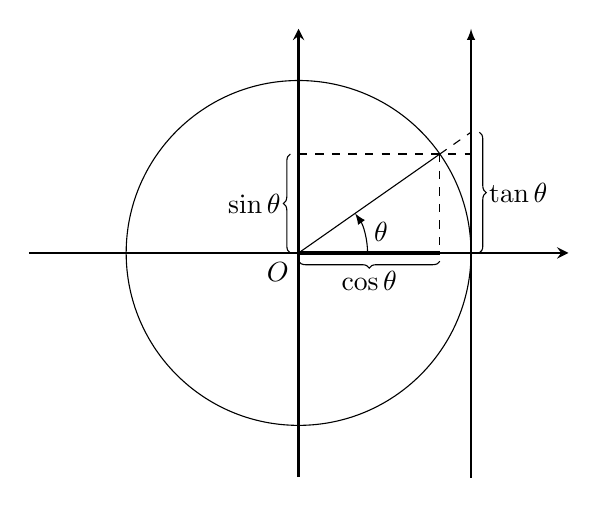
\begin{tikzpicture}
\begin{axis}[
standard,
xmin=-1, xmax=1,
ymin=-1, ymax=1,
axis equal,
xtick={\empty}, ytick={\empty},]
\draw[] (0,0) circle [radius=1];
\draw[] (0,0) -- (35:1);
\draw[dashed] (35:1) -- (35:1.2207);
\draw[-latex](1,-1.5) -- (1,1.3);
\draw[-latex] (0.4,0) arc [start angle=0, end angle=35, radius=0.4];
\node[right] at (17.5:0.4) {$\theta$};
\draw[dashed] (35:1) -- (35:1 |- 0,0);
\draw[very thick] (0,0) -- (35:1 |- 0,0);
\draw[very thick] (0,0) -- (35:1 -| 0,0);
\draw[dashed] (35:1 -| 0,0) -- (35:1 -| 1,0);
\node[below left] at (0,0) {$O$};
\draw[decoration={brace,mirror,raise=3pt},decorate] (1,0) -- (35:1.2207) node[pos=0.5, right=3pt]{$\tan\theta$};
\draw[decoration={brace,raise=3pt},decorate] (0,0) -- (35:1 -| 0,0) node[pos=0.5, left=3pt]{$\sin\theta$};
\draw[decoration={brace,mirror,raise=3pt},decorate] (0,0) -- (35:1 |- 0,0) node[pos=0.5, below=3pt]{$\cos\theta$};
\end{axis}
\end{tikzpicture}
\end{center}

\vspace{10pt}

As an elaboration to our previous definition of the trigonometric functions, Our Math Professor is now describing them as being "projections" of a line in standard position in a unit circle onto the coordinate axes. For instance, the sine of theta is the vertical projection of the line extending from the origin in standard position at angle theta until it intersects the unit circle.

\vspace{10pt}

The reason why the tangent is defined as the vertical projection of the line in standard position at an angle theta until it intersects the tangent axis is because it is the ratio of the sine and the cosine over a period of one - that's just the slope. They're the same thing, and Our Math Professor did a visual proof of this at a later point in class.

\begin{align*}
\textnormal{Sine }&=\textnormal{ vertical

projection}\\
\textnormal{Cosine }&=\textnormal{ horizontal

projection}
\end{align*}

\vspace{10pt}

Our Math Professor suggested that any student interested in the older typesetting techniques of math textbooks check out the old Wentworth Elementary textbooks in Trigonometry and Geometry.

\vspace{10pt}

It is important that the period of the tangent function is  pi; this means that the angle diametrically opposite to the angle in question has the same tangent - excluding $\pm\pi/2+k\cdot\pi:k\in\mathbb{I}$ of course (this is a bit of a fancy way of saying that the angle cannot cause the line to point straight up or down).

\vspace{10pt}

At this point, Our Math Professor did a visual proof of our previous claim that an angle's tangent being the ratio of  its vertical and horizontal projections for right triangles with acute angles of theta.

\vspace{10pt}

\begin{center}
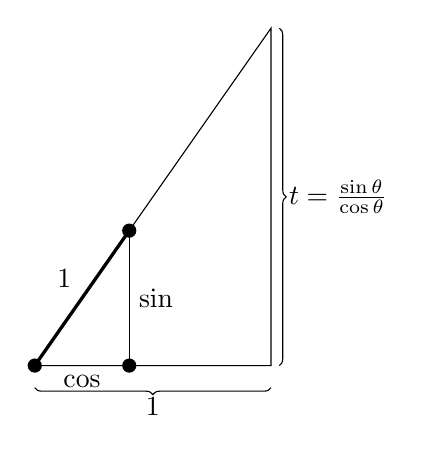
\begin{tikzpicture}[scale=3]
\coordinate (O) at (0,0);
\coordinate (P) at (1,1.4281);
\coordinate (X) at (P |- O);
\draw[] (O) -- (P) -- (X) -- cycle;
\draw[very thick] (O) -- (55:0.6974) node[pos=0.5, above left]{$1$};
\draw[] (55:0.6974) -- (55:0.6974 |- O);
\fill[] (55:0.6974) circle [radius=0.03];
\fill[] (O) circle [radius=0.03];
\fill[] (55:0.6974 |- O) circle [radius=0.03];
\path[] (O) -- (55:0.6974 |- O) node[pos=0.5,below]{$\cos$};
\path[] (55:0.6974 |- O) -- (55:0.6974) node[pos=0.5,right]{$\sin$};
\draw[decoration={brace,mirror,raise=8pt},decorate] (0,0) -- (1,0) node[pos=0.5, below=8pt]{$1$};
\draw[decoration={brace,mirror,raise=3pt},decorate] (1,0) -- (P) node[pos=0.5, right=3pt]{$t=\frac{\sin\theta}{\cos\theta}$};
\end{tikzpicture}
\end{center}

\[\left\{\begin{array}{cc}\theta\to\pi/2-\\\tan\theta\to\infty\end{array}\right.\quad\textnormal{ and }\quad\left\{\begin{array}{cc}\theta\to-\pi/2+\\\tan\theta\to-\infty\end{array}\right.\]

Again, Our Math Professor reiterated that any angle theta for which the tangent function is defined has the same tangent as the angle which is its diametric opposite. That is,

\[\tan(x+k\cdot\pi)=\tan x\]

\vspace{10pt}

We also went over the following two limits, the first of which - which states that the slope of an angle's tangent approaches one for small values of theta - directly follows from the second which is itself proved using the Sandwich Theorem or L'Hospital's Rule.

\vspace{10pt}

\begin{center}
\begin{tikzpicture}
\begin{axis}[
standard,
xmin=-1.57, xmax=1.57,
ymin=-1.57, ymax=1.57,
axis equal,
xtick={\empty}, ytick={\empty}]
\draw[dashed] (-pi/2,-3) -- (-pi/2,3);
\draw[dashed] (pi/2,-3) -- (pi/2,3);
\addplot[samples=200,domain=-1.5:1.5] {tan(x*180/pi)};
\addplot[] {x};

\end{axis}
\end{tikzpicture}
\end{center}

\vspace{10pt}

It's kind of funny to think about the tangential line to the tangent function. And we reiterate that $\tan x=x$ when $|x|$ is small.

\vspace{10pt}

\begin{center}
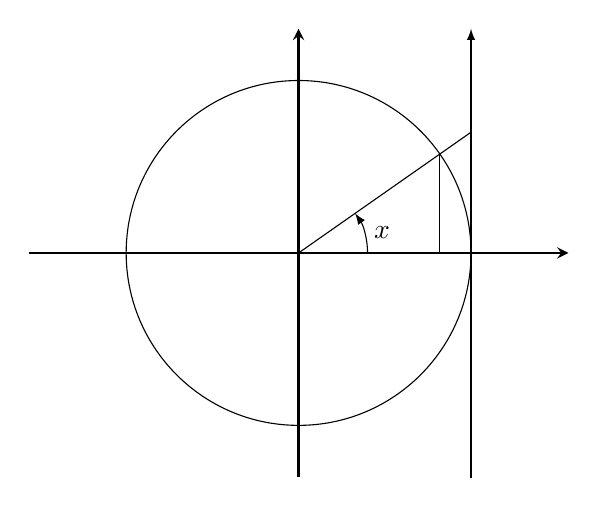
\begin{tikzpicture}
\begin{axis}[
standard,
xmin=-1, xmax=1,
ymin=-1, ymax=1,
axis equal,
xtick={\empty}, ytick={\empty}]
\draw[] (0,0) circle [radius=1];
\draw[] (0,0) -- (35:1);
\draw[] (35:1) -- (35:1.2207);
\draw[-latex](1,-1.5) -- (1,1.3);
\draw[-latex] (0.4,0) arc [start angle=0, end angle=35, radius=0.4];
\node[right] at (17.5:0.4) {$x$};
\draw[] (35:1) -- (35:1 |- 0,0);
\end{axis}
\end{tikzpicture}
\end{center}

\vspace{10pt}

As can bee seen from the picture, the angle's sine is less than its arc and both are less than its tangent;

\begin{center}
\begin{tabular}{|c|}
\hline\\
$\sin x<x<\tan x$\\[1em]
\hline
\end{tabular}
\end{center}

\vspace{10pt}

We then discussed the concept of a period of a function. For example $\sin\Rightarrow2\pi$, and $\tan\Rightarrow\pi$.

\vspace{10pt}

{\bf{}HOMEWORK} define $y=\mbox{arccot }x$, where the cotangent axis is the line $y=1$.

\vspace{10pt}

\begin{center}
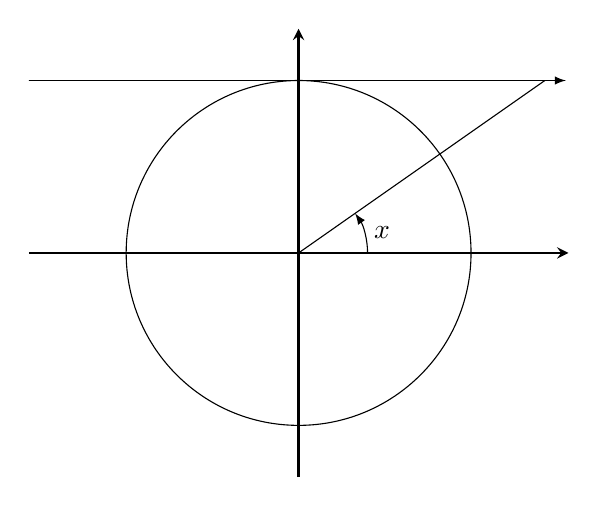
\begin{tikzpicture}
\begin{axis}[
standard,
xmin=-1, xmax=1,
ymin=-1, ymax=1,
axis equal,
xtick={\empty}, ytick={\empty}]
\draw[] (0,0) circle [radius=1];
\draw[] (0,0) -- (35:1.7434);
\draw[-latex](-1.6,1) -- (1.55,1);
\draw[-latex] (0.4,0) arc [start angle=0, end angle=35, radius=0.4];
\node[right] at (17.5:0.4) {$x$};
\end{axis}
\end{tikzpicture}
\end{center}

\vspace{10pt}

Our Math Professor also suggests we define secant and cosecant on our own for practice

\vspace{10pt}

{\bf{}EXAMPLE} Evaluate $\tan(\arctan3)$

\vspace{10pt}

 $\tan(\arctan3)=3$ because arctangent is defined for all angles of theta, and tangent can take as input any output of its vertically restricted inverse.

\vspace{10pt}

{\bf{}EXAMPLE} Evaluate $\arctan(\tan5)$

\vspace{10pt}

The way to findout how many groups of pi are in the number inside of the tangent function - if the number is large - is to divide that number by pi and subtract pi multiplied by the floor function - removes decimals - of what you get from your original number, that will be the precise number of the $-\pi/2<\theta<\pi/2$ which outputs the same value when inputted into the tangent function. 

\vspace{10pt}

Find $y:\ \tan y=\tan5$ and $|y|<\pi/2$.

\begin{center}
\begin{tikzpicture}
\begin{axis}[
scale=2,
standard,
xmin=-2, xmax=2,
ymin=-3, ymax=1,
axis equal,
xtick={\empty}, ytick={\empty}]
\draw[] (0,0) circle [radius=1];
\draw[] (0,0) -- (-73.5211:3.5253);
\draw[-latex] (1,-4) -- (1,1.6);
\draw[-latex] (0.2,0) arc [start angle=0, end angle=286.4789, radius=0.2];
\node[below left] at (225:0.2) {$5$};
\draw[-latex] (0.2,0) arc [start angle=0, end angle=-73.5211, radius=0.2];
\node[below right] at (-32.7601:0.2) {$\theta$};
\end{axis}
\end{tikzpicture}
\end{center}

\vspace{10pt}

$\tan5=\tan\theta$ because $|\theta|<\pi/2$. Therefore, $\arctan(\tan5)=-(2\pi-5)$.

\vspace{10pt}

{\bf{}EXAMPLE} Evaluate $\sin(2\arctan3)$

\vspace{10pt}

I want to just write a little blurb here to emphasize the importance of at least memorizing the trigonometric formulas if you haven't already. It can also be helpful to develop an intuition about them. For instance, $\cos(x-y)=\cos(x)\cos(y)+\sin(x)\sin(y)$ can be proven easily by setting up two angles in a unit circle, calculating the distance between their terminal points using the cosine and distance laws, then setting them equal and simplifying. But be warned, these trigonometric identities will be essential for the course, and some people will be blindsided by this after it is too late. Anyways, back to the question.

\vspace{10pt}

Recognizing a double-angle sine formula, we first let $\theta=\arctan3$.

\vspace{10pt}

What is known about theta? Well, $\tan\theta=3;\ |\theta|<\pi/2$. The tangent function is related to the sine and cosine functions - which appear after using the double angle formula, and we can use this to re-express it it in terms of sine and cosine. We can do this using Pythagoras's formula;

\begin{align*}
\sin^2\theta+\cos^2\theta&=1\\
\tan^2\theta+1&=1/\cos^2\theta\\
\cos^2\theta(\tan^2\theta+1)&=1\\
\cos^2\theta&=1/(1+\tan^2\theta)\\
\mbox{So, }\cos\theta&=(+\mbox{ or }-\mbox{ ?})1/\sqrt{1+\tan^2\theta}
\end{align*}

\vspace{10pt}

And we choose $+$, because $\cos\theta>0$ follows from $\theta\in(-\pi/2,\pi/2)$ This lets us solve for the cosine, and then the sine  by using Pythagoras's Theorem.

\[\Rightarrow\cos\theta=+1/\sqrt{1+\tan^2\theta}=1/\sqrt{1+3^2}=1/\sqrt{10}\]

\[\Rightarrow\sin2\theta=2\sin\theta\cos\theta=2\cdot\frac{3}{\sqrt{10}}\cdot\frac{1}{\sqrt{10}}=\frac{6}{10}=\frac{3}{5}\]

\vspace{10pt}

Our Math Professor notes that we will likely never have a practical reason to use $\sec^2\theta$, and that even if we do that it is better written as $1/\cos^2\theta$ for reasons of staying true to the original geometric intuition.

\vspace{10pt}

Our Math Professor reiterated our earlier point about the essentiallity of the trigonometric identities for this course, even emphasizing the tangent angle addition formula which is in the formula sheet. I really recommend at least memorizing these formulas, and if you have the time - deriving them; it is \textit{that} important.

\vspace{10pt}

{\bf{}HOMEWORK} Evaluate the following expressions;

\begin{enumerate}[label=\alph*)]
\item $\sin(\arctan(-2))$
\item $\cos(2\arctan\frac{1}{2})$
\item $\tan(2\arccos\frac{1}{3})$
\item $\tan(\arcsin\frac{1}{2}+\arccos\frac{1}{3})$
\end{enumerate}

\vspace{10pt}

We ended class with differentiating the inverse trigonometric functions, followed  by a couple inverse trigonometric formulas.

\begin{align*}
y&=\arcsin x\\
x&=\sin y\\
y^\prime&=\frac{1}{x^\prime(y)}=\frac{1}{\cos y}
\end{align*}

\vspace{10pt}

\begin{center}
What is $\cos y$ when $\left\{\begin{array}{c}\sin y=x\\|y|\leq\pi/2\end{array}\right.$?
\end{center}

\vspace{10pt}

Well, $\cos^2y+\sin^2y=1$, so $\cos y=(+\mbox{ or }-\mbox{ ?})\sqrt{1-\sin^2y}$, and we choose $+$ because $|y|\leq\pi/2$.

\[\therefore(\arcsin x)^\prime=\frac{1}{\sqrt{1-x^2}}\]

\vspace{10pt}

And the formulas we looked at are as follows;

\begin{center}
\begin{tabular}{|l|}
\hline\\
{\bf{}1.} $\arcsin x+\arccos x=\pi/2$\\[0.5em]
{\bf{}2.} $(\arcsin x)^\prime+(\arccos x)^\prime=0$\\[0.5em]
{\bf{}3.} $(\arccos x)^\prime\begin{aligned}[t]&=-(\arcsin x)^\prime\\&=-1/\sqrt{1-x^2}\end{aligned}$\\[1em]
\hline
\end{tabular}
\end{center}






\end{document}


